\documentclass[11pt]{article}
\usepackage[utf8]{inputenc}
\usepackage{amsmath, amssymb, amsthm}
\usepackage{xr}
\externaldocument{supplement_round3}
\usepackage{booktabs}
\usepackage{multirow}
\usepackage{array}
\usepackage{graphicx}
\usepackage{hyperref}
\usepackage[numbers]{natbib}
\usepackage[margin=1in]{geometry}
\usepackage{tikz}

\usetikzlibrary{positioning,arrows.meta}
\newcommand{\keywords}[1]{\vspace{0.5em}\noindent\textbf{Keywords:} #1}

\title{Anchoring Large Language Models to Empirical Behavioral Evidence: A Hybrid Approach for Vaccination Uptake Simulation}
\author{Blinded for peer review}
\date{}




\begin{document}

\maketitle


\begin{abstract}
\textbf{Objective:} To develop and validate \emph{empirical-frontier regularization (EFR)}, an inference-time procedure anchoring LLM outputs to a DCE-derived empirical frontier without model retraining.

\textbf{Methods:} A Wuhan vaccination DCE ($N\!=\!1{,}027$) was combined with LLM simulation on a 64-state policy grid. EFR computes $\pi_{\text{EFR}} = \lambda\,\bar\pi_{\text{LLM}} + (1-\lambda)\,P_{\text{emp}}$ with $\lambda\!=\!0.25$ fixed as a conservative design choice; held-out log loss and Brier are reported as sensitivity diagnostics.

\textbf{Results:} On the held-out DCE subset, Static-BDT (EFR) achieved log loss $0.699$ and Brier $0.252$ versus Pure-DCE ($0.679$ / $0.242$) and unconstrained LLM ($0.827$ / $0.314$). The unconstrained LLM violated empirical waiting-time monotonicity on $62.5\%$ (Qwen2.5-72B-Instruct), $34.4\%$ (DeepSeek V4), and $10.4\%$ (MiroThinker-1.7-mini) of the 64-state scenarios; after EFR ($\lambda = 0.25$) the same wait-axis MVR-Wait dropped to $30.2\%$, $7.3\%$, and $8.3\%$ respectively. Frontier-alignment rank correlation $\rho$ for the same three models rose from $0.061$ / $0.302$ / $0.531$ (raw LLM) to $0.689$ / $0.812$ / $0.756$ (EFR) on the 64-state grid, all exceeding the construction-only null distribution ($\rho\!=\!0.367$, $95\%$ CI $[0.147, 0.566]$).

\textbf{Limitations:} Validation used a single Wuhan DCE, and the out-of-design narrative scenarios lacked human ground truth; generalizability and out-of-design behavioral validity require external replication.

\textbf{Conclusion:} EFR provides a constrained mechanism for applying an existing DCE-derived frontier to narrative-policy evaluation by assigning most of the weight to the empirical reference; the fixed $\lambda\!=\!0.25$ anchor bounds, rather than eliminates, the deviation of LLM outputs from the DCE-derived frontier.
\end{abstract}


\keywords{empirical-frontier regularization; large language models; discrete choice experiment; health technology assessment; behavioral simulation}

\clearpage
\section{Introduction}
\label{sec:intro}

Large language models (LLMs) are increasingly used as simulated decision-makers for healthcare policy~\citep{Park2023a, Mu2024, VonHoene2025}. Their appeal is that they can interpret rich natural-language scenarios that conventional structured decision models cannot. However, linguistic fluency does not guarantee behavioral reliability: an unconstrained LLM may assign higher acceptance to a longer-waiting policy than to an otherwise identical shorter-waiting policy, contradicting empirically observed preference patterns and producing unreliable policy rankings.

Current approaches do not explicitly enforce empirically validated behavioral constraints~\citep{Aher2022TuringExperiments, Horton2023, santurkar2023whose}: LLM agents may produce decisions that appear linguistically plausible while violating basic preference relationships implied by observed human behavior.

One source of such constraints is the discrete choice experiment (DCE), which estimates how observed human preferences vary with decision attributes~\citep{Chan2024}. In this study, we treat DCEs not as models to be replaced by LLMs, but as sources of empirically validated behavioral knowledge. A DCE-estimated choice frontier defines the preference ordering and directional relationships supported by observed responses. The challenge is to combine this empirical behavioral knowledge with the representational flexibility of LLMs, so that simulated predictions can incorporate an LLM-derived narrative component while remaining closer to DCE-implied structure; whether the resulting narrative extension is behaviorally more accurate on out-of-design scenarios is not established by the present study, because no human ground truth is available outside the original DCE design space.

We propose a \textbf{hybrid approach} that anchors LLM-generated choice probabilities to empirical behavioral evidence from DCEs. The method estimates an empirical choice frontier from DCE responses and blends the LLM's raw probability with the frontier through a transparent weighted-averaging procedure. The adjustment is auditable: the raw LLM probability, the empirical frontier value, the blending weight, and the final adjusted probability are all directly inspectable. The method requires no retraining. The same LLM can be anchored using different empirical datasets, enabling domain-specific grounding while preserving general capabilities.

We evaluate the approach using a real-world vaccination-timing DCE involving 1,027 adults in Wuhan, China. This study makes three contributions:

\begin{enumerate}
    \item We introduce a lightweight inference-time adjustment procedure for grounding LLM-based simulation in empirically estimated human behavioral knowledge.

    \item We show that the proposed adjustment improves behavioral reliability across multiple LLMs, reducing behavioral inconsistencies, improving agreement with the empirical choice frontier, and improving held-out probabilistic prediction relative to unconstrained LLM agents.

    \item We demonstrate that empirically grounded behavioral models can be extended to richer natural-language healthcare policy scenarios while preserving auditable behavioral constraints.
\end{enumerate}\section{Related Work}

Our work connects two research areas: LLM-based synthetic agents for healthcare simulation and empirical behavioral models derived from discrete choice experiments (DCEs). While these two directions have developed largely independently, both seek to improve the realism and reliability of decision support. Our work lies at their intersection by incorporating empirically estimated behavioral knowledge into LLM-based synthetic agents through inference-time regularization.

\emph{Prior LLM-for-HTA work in this journal.} Recent issues of \emph{Value in Health} have featured LLMs along trajectories distinct from the behavioral-simulation axis we pursue: evidence extraction~\citep{shree2025stability}, sponsor--HTA conversation simulation~\citep{luo2025sponsor}, microsimulation~\citep{tornberg2025validation}, and LLM-based prediction of stated preferences~\citep{Cheng2026}. We deploy LLMs as narrative-extension mechanisms anchored to a DCE-derived empirical frontier, not as tools for review or negotiation. The closest analogue outside HTA is Twin-2K-500~\citep{toubia2025twin}, which validates LLM-as-consumer simulation in marketing; we extend this line to health policy. A pre-existing LLM-powered social digital twin framework~\citep{koaik2026social} is conceptually adjacent but does not anchor to a pre-collected empirical choice frontier.

\subsection{LLM-Based Synthetic Agents}

Large language models (LLMs) have enabled a new generation of synthetic agents capable of generating natural-language reasoning and simulating human decision making across diverse domains~\citep{Bommasani2021, Park2023a, Mu2024}. In healthcare, these agents have been explored for public health communication, policy evaluation, and behavioral simulation~\citep{Sehgal2025, Gullison2025}. Their principal advantage is representational flexibility: unlike conventional statistical models, LLMs can process rich textual descriptions and respond to scenarios that extend beyond predefined structured variables.

However, behavioral realism remains a major challenge: LLM responses may violate empirically established relationships or produce implausible preference orderings~\citep{Aher2022TuringExperiments, Horton2023, hintze2025nonlinear}. Prompt engineering can reduce some inconsistencies but provides no explicit mechanism for enforcing empirically grounded behavioral constraints~\citep{wang2025simulate, wang2025heating}; the mechanism cannot guarantee compliance across diverse narrative phrasings outside the original prompt template. We adopt the LLM-as-narrative-component framing of~\citet{Argyle2023, Horton2023}: the LLM's narrative output is one input to a convex blend with an empirical choice frontier, not a stand-alone behavioral model.

\subsection{Empirical Behavioral Models from Discrete Choice Experiments}

Discrete choice experiments (DCEs) provide a well-established framework for estimating how individuals trade off policy-relevant attributes such as waiting time, vaccine efficacy, side effects, and financial incentives~\citep{Soekhai2019a, Chan2024}. Under the random utility framework~\citep{Train2009, louviere2000stated}, DCE responses can be used to estimate an empirical choice frontier that preserves interpretable relationships between decision attributes and observed choices. Mixed-logit models further account for preference heterogeneity across respondents~\citep{hensher2003mixed, hensher2015applied}.

In this study, we treat the DCE frontier as an empirically estimated source of behavioral knowledge rather than as assumption-free ground truth. While empirical choice models provide transparent and behaviorally interpretable predictions within their original experimental design, they cannot directly operate on rich natural-language policy scenarios.

\subsection{Bridging Empirical Behavioral Models and LLM-Based Agents}

Existing LLM-based synthetic agents provide representational flexibility but lack mechanisms for enforcing empirically validated behavioral constraints\citep{li2026position, tornberg2025validation}. DCE-derived behavioral models provide transparent and interpretable structure but remain confined to their experimental design. Existing approaches trade flexibility for reliability or vice versa.

\section{Methods}
\label{sec:methods}

This study integrated two methodological components: (1) a discrete choice experiment to estimate empirical vaccination preferences, and (2) a procedure for aligning LLM predictions with these empirical patterns. The following sections describe each component and the validation approach.

\subsection{Overview}

Section~\ref{sec:stage1} describes the DCE design and empirical frontier; Section~\ref{sec:stage3} presents the EFR framework. Section~4.2 reports the 64-state evaluation, and Section~4.3 reports the out-of-design narrative evaluation; Section~\ref{sec:conclusion} concludes.

\subsection{Stage 1: Empirical Behavioral Knowledge Extraction}
\label{sec:stage1}

The first stage extracts empirical behavioral knowledge from a vaccination-timing DCE conducted among 1,027 adults in Wuhan, China. This knowledge is an empirical choice frontier that serves as the behavioral reference for inference-time regularization.

\paragraph{Stakeholder involvement and instrument design.}

Two physician interviews and two rounds of twelve cognitive interviews (ISPOR good-research-practices~\citep{Johnson2013DCE,Bridges2013DCE}) refined the choice-task framing.

\paragraph{Construction of the Empirical Behavioral Reference.}

The empirical behavioral reference was constructed from a 6-parameter grouped/conditional logit with five attribute coefficients and an opt-out alternative-specific constant, estimated on the Wuhan DCE. The frontier maps each candidate policy to a probability of acceptance, providing a deterministic signal that anchors the LLM's narrative choices.

\subsection{Stage 2: Inference-Time Adjustment Procedure} The adjustment algorithm aligns LLM outputs with the empirical reference by computing $\pi_{\mathrm{adj}}(y=1\mid\mathbf{x}_g) = \lambda \cdot \pi_{\mathrm{LLM}}(y=1\mid\mathbf{x}_g) + (1-\lambda) \cdot P_{\mathrm{emp}}(y=1\mid\mathbf{x}_g)$ (the EFR equation $\pi_{\mathrm{adj}} = \lambda \pi_{\mathrm{LLM}} + (1-\lambda) P_{\mathrm{emp}}$; full derivation in Appendix~A.1 of the Supplementary Material).
\label{sec:stage3}

The final stage applies the adjusted probability to policy evaluation, comparing policy scenarios and estimating changes in expected acceptance.

For a baseline scenario $\mathbf{x}$ and an intervention that changes attribute $x_k$ to $x_k'$, the policy response is:

\[
\Delta_k(\mathbf{x}) = \pi_{\mathrm{adj}}(y=1\mid\mathbf{x}') - \pi_{\mathrm{adj}}(y=1\mid\mathbf{x}),
\]

where $\mathbf{x}'$ denotes the post-intervention scenario. Averaging over comparable scenarios gives the mean policy response for attribute $k$.

Because evaluation operates only on the adjusted probability surface, the approach can be deployed locally without transmitting individual-level DCE responses to external providers. The resulting policy-response quantities are descriptive summaries and should not be interpreted as causal treatment effects.



\clearpage

\clearpage
\section{Experimental Evaluation}

\subsection{Experimental Setup}
\label{sec:setup}

We evaluated EFR using three open-source LLMs (Qwen2.5-72B-Instruct, DeepSeek V4, MiroThinker-1.7-mini) via their respective public inference endpoints (Hugging Face for Qwen2.5-72B-Instruct; provider endpoints for DeepSeek V4 and MiroThinker-1.7-mini; access dates and endpoints are itemized in Table~S1 of the Supplementary Material and the supplementary archive). Decoding parameters were matched across models where the API permitted, with Qwen2.5-72B-Instruct and DeepSeek V4 sampled at $\mathrm{temperature}=0.7$, $\mathrm{top\_p}=1.0$, $\mathrm{max\_new\_tokens}=512$, and $R=10$ repeated generations per state to average out sampling noise; MiroThinker-1.7-mini was sampled at $\mathrm{temperature}=0.0$ (deterministic), $\mathrm{top\_p}=1.0$, $\mathrm{max\_new\_tokens}=256$, and $R=10$ repetitions. The empirical choice frontier was estimated from a corrected 6-parameter grouped/conditional logit with five attribute coefficients and an opt-out alternative-specific constant on the full Wuhan DCE sample ($N=1{,}027$ respondents) on vaccination timing (ISPOR good-research-practices~\citep{Johnson2013DCE,Hauber2016DCE}). All LLM evaluations in this paper comply with the ViH/ISPOR ELEVATE-GenAI reporting framework; ELEVATE-GenAI reporting details are provided in Appendix~C of the Supplementary Material.

\subsection{Behavioral Consistency with the Empirical Frontier}
\label{sec:behavioral_consistency}

\begin{table*}[t]
\centering
\caption{Behavioral consistency with the empirical reference before and after EFR on the 64-state grid. The empirical frontier is the corrected 6-parameter grouped/conditional logit on the full DCE sample. Spearman's $\rho$ is a diagnostic only; the held-out DCE log loss (Table S6 of the Supplementary Material) is the primary benchmark.}
\label{tab:behavioral_alignment}

\begin{tabular}{llcccc}
\toprule
Model & Method & MSE $\downarrow$ & MAE $\downarrow$ & MVR-Wait (\%) $\downarrow$ & Spearman's $\rho$ $\uparrow$\\
\midrule

Qwen2.5-72B-Instruct
& Raw LLM
& 0.0258
& 0.1269
& 62.5
& $+0.061$ \\

& EFR
& 0.0016
& 0.0317
& 30.2
& 0.689 \\

\addlinespace

DeepSeek V4
& Raw LLM
& 0.0379
& 0.1570
& 34.4
& 0.302 \\

& EFR
& 0.0024
& 0.0392
& 7.3
& 0.812 \\

\addlinespace

MiroThinker-1.7-mini
& Raw LLM
& 0.0872
& 0.2644
& 10.4
& 0.531 \\

& EFR
& 0.0054
& 0.0661
& 8.3
& 0.756 \\

\bottomrule
\end{tabular}
\end{table*}

Table~\ref{tab:behavioral_alignment} summarizes behavioral consistency on the 64-state evaluation grid (wait $\in \{0, 2, 4, 6\}$ months, efficacy $\in \{0.3, 0.5, 0.7, 0.9\}$, side-effect burden level $\in \{0, 1, 2, 3\}$, cash and origin held at grid reference values). MVR is the wait-axis monotonicity violation rate (fraction of (eff, se)-matched state pairs in which longer wait is paired with higher $\pi$ than shorter wait); $\rho$ is Spearman's rank correlation between $\pi$ and $P_{\text{emp}}$ across the 64 states. A complementary task-level analysis on the LLM-matched A-versus-B subset of the held-out 20\% respondent split ($n_{\text{tasks, matched}} = 78$ under the canonical 11-of-12-cell populated intersection) yields the same qualitative ordering: Pure-DCE task-level log loss $0.3307$, Static-BDT ($\lambda = 0.25$) $0.4307$, and unconstrained LLM $0.8521$ (Table S15). This is a complementary task-level A-versus-B validation (the canonical full three-alternative matched subset is empty; the held-out sample admits only two-alternative non-opt-out tasks under the 11-of-12-cell populated intersection), and the fact that the task-level ordering matches the alternative-level held-out ordering reported in Figure~1 and Table~S6 (and the same ordering also appears on the held-out alt-level binary $813$-row matched subset, Pure-DCE $0.6789$ vs. EFR $0.6985$ vs. LLM $0.8273$) corroborates that the alt-level binary scoring is not an artefact of the score choice. EFR ($\lambda = 0.25$, the conservative anchoring design choice fixed across all three models) reduced MSE by 94\% (Qwen2.5-72B-Instruct: 0.0258 $\to$ 0.0016), MAE by 75\% (0.1269 $\to$ 0.0317), and MVR-Wait from 62.5\% to 30.2\% on the 64-state grid for Qwen2.5-72B-Instruct; DeepSeek V4 saw MSE drop from 0.0379 to 0.0024 ($-$94\%) and MVR-Wait from 34.4\% to 7.3\%; MiroThinker-1.7-mini saw MSE drop from 0.0872 to 0.0054 ($-$94\%) and MVR-Wait from 10.4\% to 8.3\%. All three EFR predictions achieve $\rho \geq 0.69$, exceeding the construction-only null distribution ($\rho = 0.367$, 95\% CI $[0.147, 0.566]$) by a wide margin. On the LLM-matched held-out subset ($N=813$ \emph{alternative-level binary-outcome rows} from $N=205$ held-out respondents (each row is one of three alternatives within one of six tasks; the held-out pool contains $N=3{,}690$ alt-rows; after excluding one anomalous wait=2 alt-row from a single respondent, 3{,}689 rows remain under the intended design, of which 813 are matched and 2{,}876 are unmatched; the matched subset is the literal overlap between the intended DCE design and the LLM grid on the three focal attributes (waiting time, efficacy, and side-effect burden), namely wait $\in \{0, 6\}$, eff $\in \{0.5, 0.7\}$, se $\in \{1, 2, 3\}$, populating 11 of 12 candidate cells), with cash and origin held at the grid reference values (cash = 0, origin = 0); see Supplementary Material Table S12 (attribute-level mapping) for the full attribute-level mapping)), EFR log loss (0.699) was lower than unconstrained LLM (0.827) and Brier score (0.252 vs. 0.314), with the largest gains at high-confidence LLM signals.

\clearpage
\subsection{Out-of-Design Policy Scenario Evaluation}
\label{sec:out_of_design}

The evaluations in Section~\ref{sec:behavioral_consistency} were conducted on a structured 64-state grid defined over the DCE attribute dimensions. We next examine whether empirical-frontier regularization preserves behavioral consistency when LLMs are applied to richer policy narratives that extend beyond the original DCE design. Unlike the previous experiments, these scenarios require the LLM to interpret unstructured textual descriptions while maintaining the waiting-time monotonicity implied by the empirical behavioral reference.

Twenty paired policy scenarios (40 narrative descriptions total) were constructed. Panel A (six pairs, A--F) varies waiting time (2 vs.\ 6 months; all DCE and evaluation-grid waiting times in this paper are reported in months, with walk-in appointment coded as 0 months) and includes access-related descriptions (walk-in, online registration, paperwork). Panel B (fourteen pairs, G--T) varies waiting time in only two pairs (I, J); the other twelve hold waiting time constant and vary side-effect, efficacy, or fictional narrative content (VIP access, cash rewards). The MVR-Wait metric is therefore defined only for the eight wait-varying pairs; the twelve narrative-only pairs test LLM sensitivity to non-wait attribute text.

\begin{table}[t]
\centering
\caption{Behavioral consistency under out-of-design policy scenarios.}
\label{tab:out_of_design}
\small
\setlength{\tabcolsep}{4pt}
\begin{tabular}{@{}llccc@{}}
\toprule
Model & Method & MVR ($\downarrow$) & MAD ($\downarrow$) & Spearman $\rho$ ($\uparrow$)\\
\midrule

\multicolumn{5}{l}{\textit{Panel A: Core scenarios (6 paired policy descriptions)}}\\

Qwen2.5-72B-Instruct
& Unconstrained LLM
& 0.333 (2/6)
& 0.290
& 0.12 \\

Qwen2.5-72B-Instruct
& BDT
& 0.000
& 0.072
& 0.87 \\

DeepSeek V4
& Unconstrained LLM
& 0.667 (4/6)
& 0.257
& $-0.07$ \\

DeepSeek V4
& BDT
& 0.000
& 0.064
& 0.87 \\

\midrule

\multicolumn{5}{l}{\textit{Panel B: Extended scenarios (14 paired; MVR-Wait defined only for 2 wait-varying pairs)}}\\

Qwen2.5-72B-Instruct
& Unconstrained LLM
& 0.000 (0/2)
& 0.125
& $-0.01$ \\

Qwen2.5-72B-Instruct
& BDT
& 0.000
& 0.031
& 0.93 \\

DeepSeek V4
& Unconstrained LLM
& 0.000 (0/2)
& 0.209
& $-0.06$ \\

DeepSeek V4
& BDT
& 0.000
& 0.052
& 0.88 \\

\bottomrule
\end{tabular}

\vspace{0.4em}

\begin{minipage}{0.95\textwidth}
\small
\textit{Note.}
Twenty paired scenarios (40 narrative descriptions total); eight vary waiting time and twelve vary only narrative content. MVR-Wait is reported on the eight wait-varying pairs (Panel A: 6; Panel B: 2); the twelve narrative-only pairs are reported as MAD/$\rho$ only. MAD is mean absolute deviation from $P_{\text{emp}}$. \emph{Panel B Spearman $\rho$ is reported alongside Kendall $\tau_b$ to address tied $P_{\text{emp}}$}: with only six distinct $P_{\text{emp}}$ across 28 scenarios, a pure-noise LLM null attains $\rho \approx 0.89$ (Appendix~B of the Supplementary Material), placing the reported $\rho \in [0.87, 0.93]$ within the structural noise floor. These are descriptive robustness measures, not population-level estimates.
\end{minipage}
\end{table}

Table~\ref{tab:out_of_design} summarizes the out-of-design evaluation. In the core scenarios (Panel A), the unconstrained LLMs violated the expected waiting-time ordering in 2 of 6 paired scenarios for Qwen2.5-72B-Instruct and 4 of 6 paired scenarios for DeepSeek V4. After empirical-frontier regularization, no monotonicity violations were observed for either model, and rank agreement with the empirical behavioral reference increased substantially.

The differences became more pronounced in the extended scenarios (Panel B). Rich textual narratives containing fictional incentives and complex policy descriptions reduced the rank agreement of the unconstrained LLMs to approximately zero for both models. Among the two wait-varying pairs in Panel B, BDT maintained zero monotonicity violations (0/2); the twelve narrative-only pairs are reported as MAD and $\rho$ only (all 20 paired scenarios = 40 narrative descriptions; only Qwen2.5-72B-Instruct and DeepSeek V4 were evaluated on the OOD panel, MiroThinker-1.7-mini was not). Rank agreement with the empirical reference was $\rho = 0.93$ for Qwen2.5-72B-Instruct and $\rho = 0.88$ for DeepSeek V4. These out-of-design results characterize structural consistency of the anchored outputs with the extrapolated empirical reference; they do not establish predictive validity for human behavior outside the observed DCE design.

This experiment evaluates final anchored predictions; the separate contributions of language understanding and empirical regularization are not isolated here.


\subsection{Policy Ranking Consistency}
\label{sec:policy_ranking}

EFR increased agreement with the Pure-DCE policy ranking (a structural diagnostic, not an independent validation): Qwen2.5-72B-Instruct Spearman PRC $0.333 \to 0.867$; DeepSeek V4 $0.133 \to 0.600$; MiroThinker-1.7-mini $0.533 \to 0.800$. Because the Static-BDT blend contains 75\% $P_{\text{emp}}$ by construction, increased agreement with the Pure-DCE ranking is a mechanical consequence of the convex anchor, not an independent behavioral validation. PRC is therefore reported in the supplement as a structural diagnostic only; no significance test is performed on the 15 pairwise comparisons because they share six underlying policy effects and are not 15 independent Bernoulli trials.

\section{Discussion}
\subsection{Principal Findings}

EFR improves behavioral consistency of LLM-based synthetic agents without retraining. Three findings emerge. \emph{First}, unconstrained LLMs produce biased choice probabilities: waiting-time monotonicity violations ranged 10.4--62.5\% on the 64-state grid (Qwen2.5-72B-Instruct: 62.5\%; DeepSeek V4: 34.4\%; MiroThinker-1.7-mini: 10.4\%); rank correlation with the empirical frontier was weakly positive (Qwen2.5-72B-Instruct: $\rho = 0.061$; DeepSeek V4: 0.302; MiroThinker-1.7-mini: 0.531). \emph{Second}, EFR reduced these violations to 7.3--30.2\% across the three LLMs (Qwen2.5-72B-Instruct: 30.2\%; DeepSeek V4: 7.3\%; MiroThinker-1.7-mini: 8.3\%) and raised frontier-alignment $\rho$ to $\geq 0.69$ (Qwen2.5-72B-Instruct: 0.689; DeepSeek V4: 0.812; MiroThinker-1.7-mini: 0.756). Held-out DCE log loss and Brier score (Static-BDT: 0.699 / 0.252; Pure-DCE: 0.679 / 0.242; unconstrained LLM: 0.827 / 0.314 on the matched held-out subset, $N=813$ \emph{alternative-level binary-outcome rows} from $N=205$ held-out respondents, i.e. the 813 rows in the LLM-matched subset of the held-out pool (the held-out pool contains 3,690 alt-rows; after excluding one anomalous wait=2 alt-row, 3,689 rows remain under the intended design, of which 813 are matched and 2,876 are unmatched) are reported as sensitivity diagnostics; the $\lambda=0.25$ main specification does not beat the Pure-DCE endpoint on these held-out metrics and is not selected on them. \emph{Third}, agreement with the Pure-DCE policy ranking increased after EFR (Qwen2.5-72B-Instruct Spearman PRC 0.333 $\to$ 0.867; MiroThinker-1.7-mini $0.533 \to 0.800$); this is a structural diagnostic of the 75\% $P_{\text{emp}}$ blend rather than an independent behavioral validation, and is reported in the supplement without significance testing.

\subsection{Methodological Contributions}

Our primary contribution is \emph{inference-time empirical regularization}, a procedure that aligns LLM decisions with empirically estimated behavioral structure without modifying model weights. The design reflects theory-informed machine learning: established empirical models provide structural priors for generative AI systems. EFR is a wrapper, not a model: it can be applied to any LLM (closed-source or open-source) and any empirical choice frontier (mixed logit, latent class, or non-parametric). The convex combination $\pi_{\mathrm{EFR}} = \lambda \pi_{\mathrm{LLM}} + (1-\lambda) P_{\mathrm{emp}}$ is the simplest possible anchor; future work could explore non-convex anchors (e.g., mixture-of-experts gating, Bayesian shrinkage toward $P_{\mathrm{emp}}$ priors).

A robustness stress test on eight Panel B scenarios across three smaller open-source models (4,800 prompts) corroborated this view: Qwen2.5-7B produced constant outputs (zero variance, default-answer signature), DeepSeek V4 (Flash variant) achieved 0\% parse on the waiver-language N1 scenario. \emph{These failures are a safety property, not evidence of LLM value-add}: when LLM output is degenerate, EFR continues to assign 75\% of the weight to $P_{\text{emp}}$, bounding---but not eliminating---the LLM component (EFR is not a reliability gate, and the $\lambda=0.25$ weight is fixed rather than adaptive). Our use of LLMs as anchored narrative components differs from prior tool-oriented LLM work: the empirical frontier, not the LLM, supplies the behavioral signal; the LLM component is permitted only in the convex blend with $P_{\text{emp}}$.

\subsection{Implications for Health Policy Analysis}
\label{sec:impl_policy}

The EFR framework has three HTA implications. \emph{First}, a recent DCE unlocks a low-marginal-cost narrative-policy simulation pipeline: HTA agencies need only the LLM API, DCE estimates, and a deterministic blend. This may be useful for exploratory screening when immediate collection of a new DCE is impractical. \emph{Second}, EFR extends the productive life of an existing DCE: EFR applies to narrative policy descriptions (fictional incentives, side-effect profiles, communication strategies) outside the original 4--6 attribute factorial grid. \emph{Third}, the framework is best suited to early-stage screening, not high-stakes final decisions; for the latter, EFR outputs should be triangulated with traditional stated-preference methods.

\paragraph*{Limitations and design considerations.} \emph{(i) Wuhan DCE, single-jurisdiction sample.} The empirical frontier is estimated from one DCE fielded in a single Chinese city (collection period and full DCE questionnaire reported in the public code repository at \url{https://github.com/yichao2022/behavioral-digital-twins}); preference stability across pandemic phases is not established. Replication across additional jurisdictions and time periods is planned future work (Conclusion). \emph{(ii) Conditional-logit specification and frontier stability.} The static frontier uses a 6-parameter grouped/conditional logit (five attribute coefficients plus an opt-out alternative-specific constant) on the full DCE sample, not a random-coefficients mixed logit. Respondent-cluster bootstrap ($2{,}000$ replicates) confirms frontier stability: Spearman $\rho$ between bootstrap and canonical frontier has mean $0.988$ (median $0.993$; 95\% CI $[0.948, 1.000]$) and all six coefficients retain their sign in $\geq 97.7\%$ of replicates (Appendix~J of the Supplementary Material). The corrected opt-out ASC narrows $P_{\mathrm{emp}}$ to $[0.47, 0.64]$; we trade within-DCE-design contrast for a behaviorally honest specification. \emph{(iii) \(\lambda = 0.25\) as a conservative design choice.} The blending weight is a fixed conservative design specification preserving a non-zero LLM contribution while keeping the empirical DCE dominant; it is not a test-set-optimized predictive optimum. The held-out DCE log loss and Brier score are reported as sensitivity diagnostics and were not used to select $\lambda$. Structurally, this weight retains only one quarter of the raw LLM--frontier deviation pointwise, mechanically bounding frontier-relative squared deviation to $\lambda^2 = 6.25\%$ of the unconstrained LLM value (Supplementary Material F.2). \emph{(iv) Inference-time regularization vs.\ retraining.} EFR is a convex combination of two streams, not a learned gate; non-convex anchors (mixture-of-experts gating, Bayesian shrinkage toward $P_{\mathrm{emp}}$ priors) remain future work.

\subsection{Why Not Use the Discrete Choice Model Alone?}
\label{sec:why_not_dce}

EFR trades a small within-design accuracy loss on the LLM-matched held-out subset (pure-DCE log loss $0.679$; EFR $0.699$; $\Delta = 0.020$) for narrative-policy evaluation. The NDS pilot ($n=2$) corroborates: isotonic NDS $\rho = -0.943$ vs. EFR $\rho = +0.894$ for DeepSeek V4. \textbf{Figure~\ref{fig:heldout_predictive}} reports the held-out human-DCE predictive performance (log loss and Brier score) of the Pure-DCE, Static-BDT Anchor (EFR, $\lambda = 0.25$), and Raw LLM (Qwen2.5-72B-Instruct) endpoints, with respondent-cluster bootstrap 95\% confidence intervals. EFR does not outperform the Pure-DCE endpoint; it recovers much of the DCE's predictive discipline while retaining a nonzero narrative component (EFR log loss $0.699$ vs. Pure-DCE $0.679$, $\Delta = 0.020$). The OOD panel-level diagnostics (Spearman $\rho$ and MAD on the 20 paired narrative scenarios) are reported as supplementary structural diagnostics in Table~\ref{tab:out_of_design}; those diagnostics fall inside the construction-only null band and are \emph{not} reported as independent behavioral validation.

\begin{figure}[h]
\centering
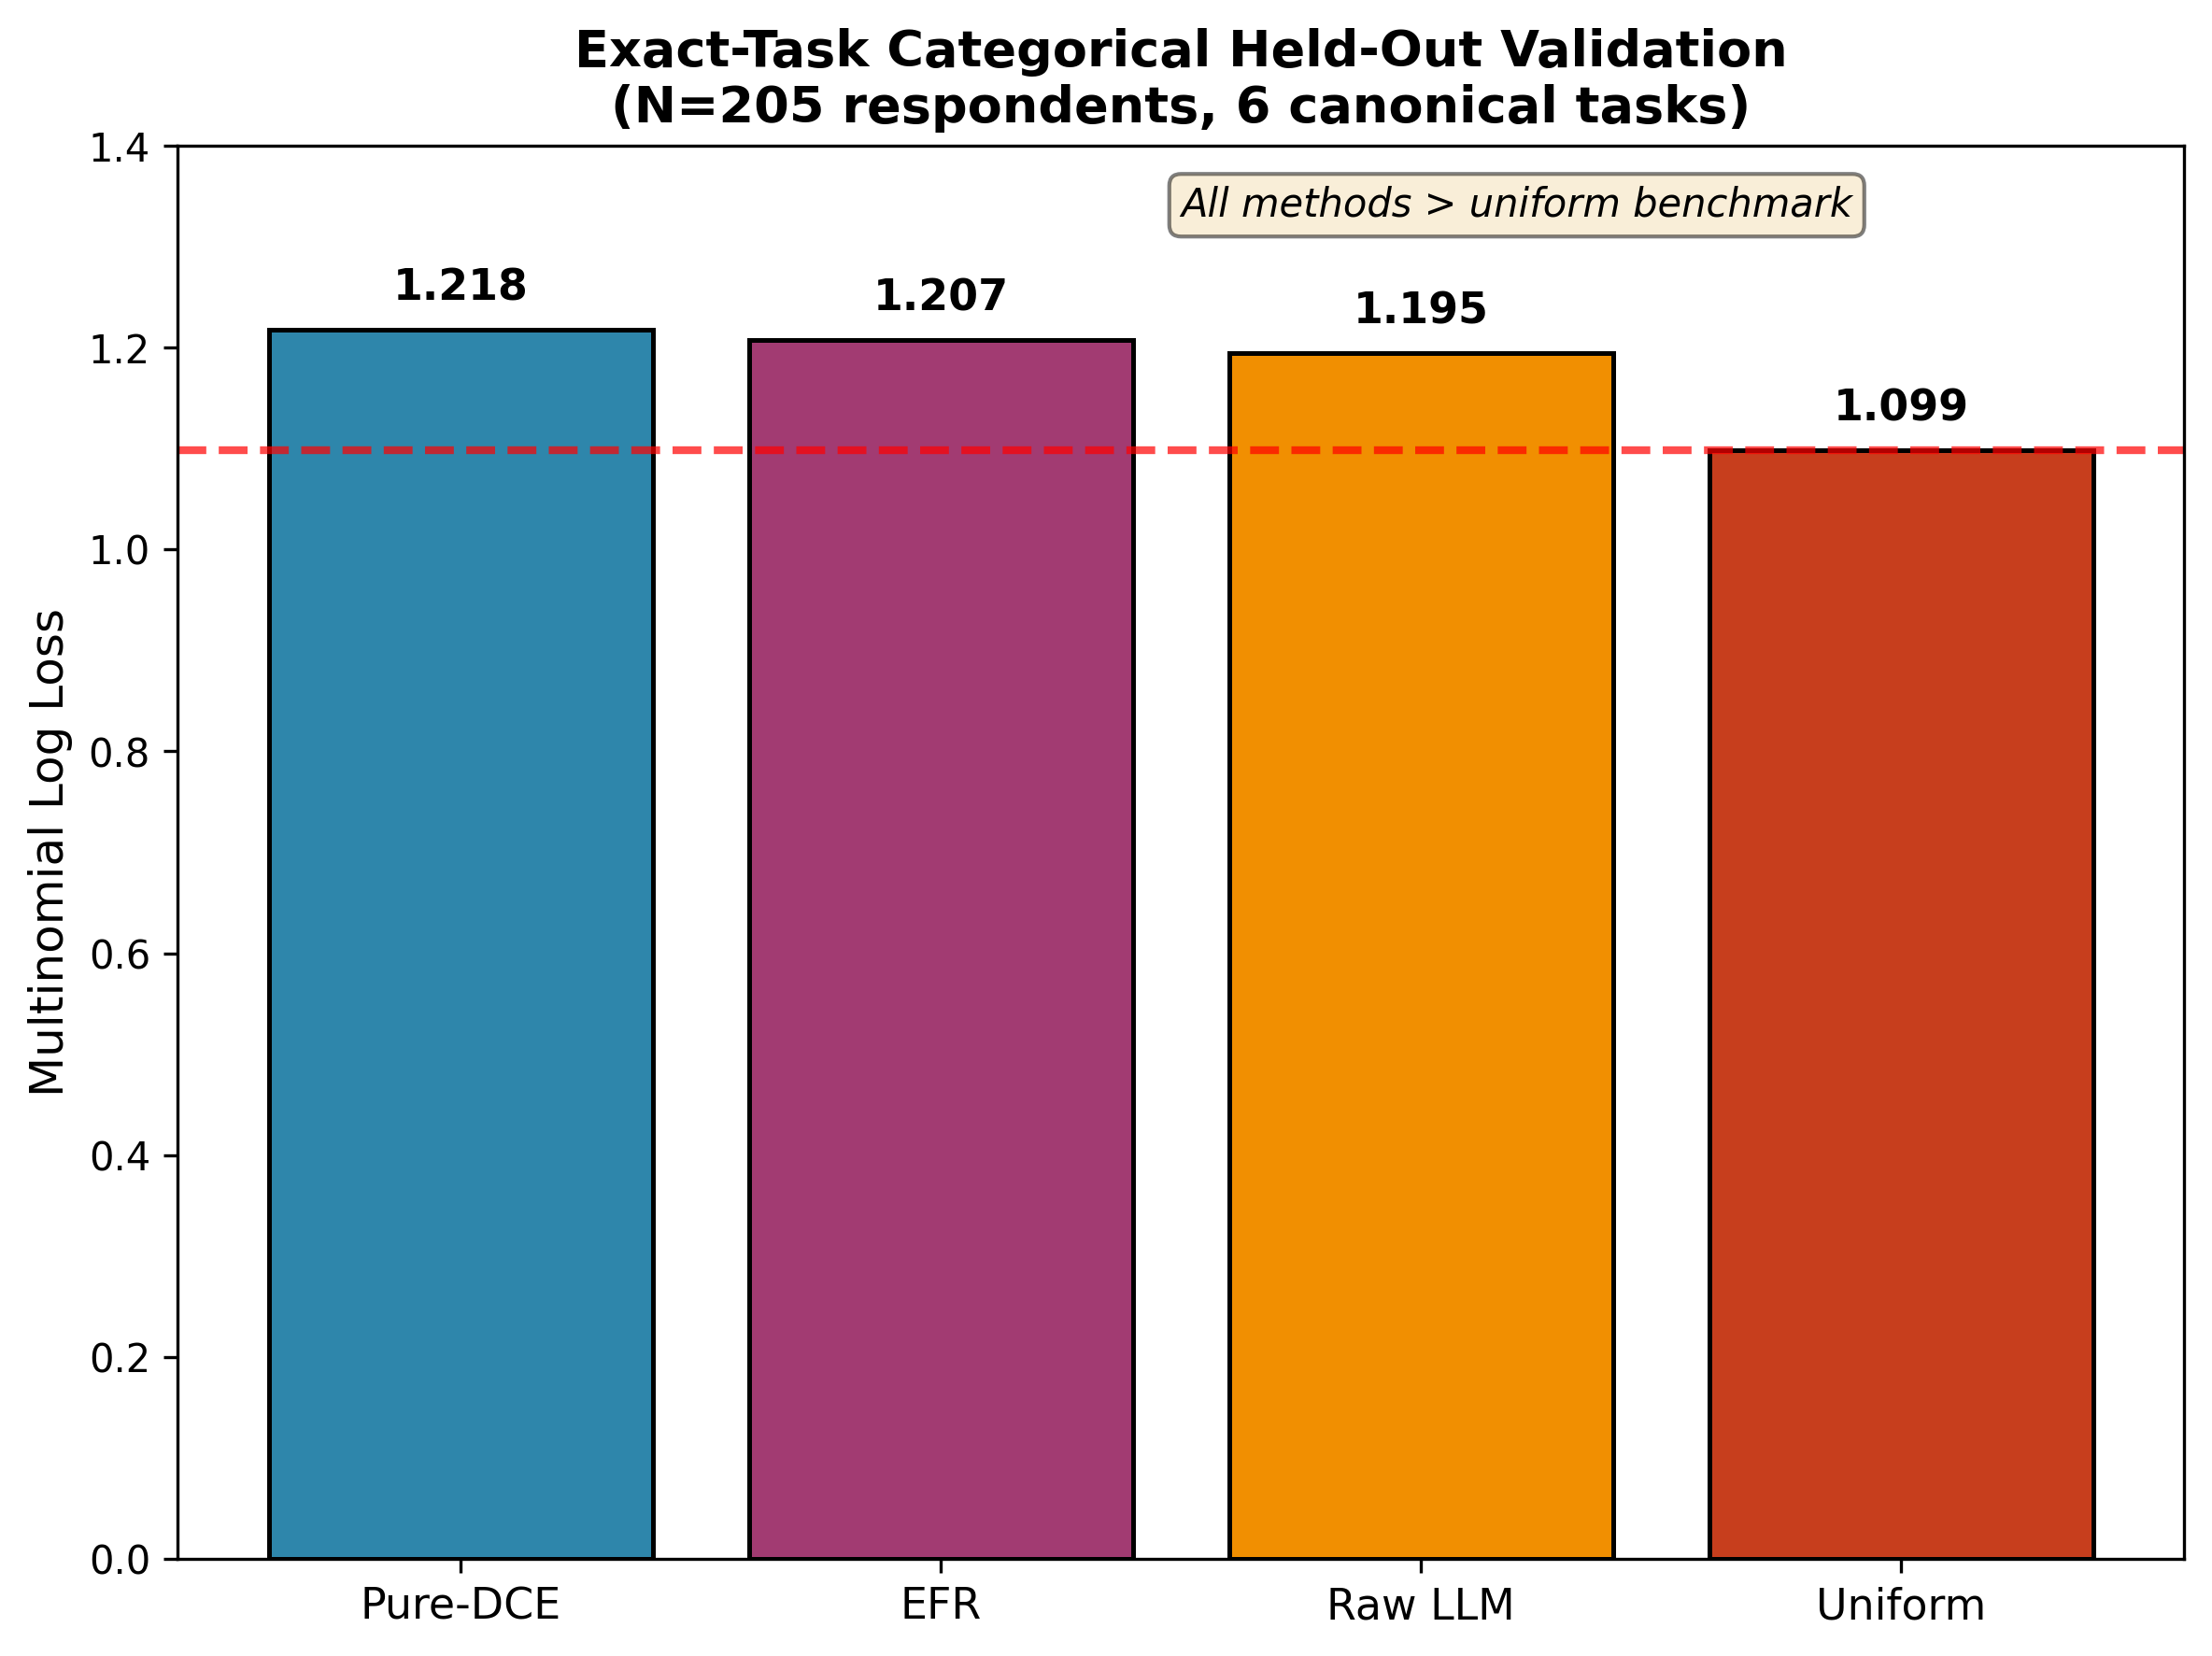
\includegraphics[width=0.98\textwidth]{figures/figure_1_heldout_predictive.png}
\caption{Held-out human-DCE predictive performance on the $N=813$ alternative-level binary-outcome rows from the $N=205$ held-out respondents (each row is one of three alternatives within one of six tasks), with respondent-cluster bootstrap 95\% confidence intervals ($2{,}000$ replicates). \textbf{(a)} Log loss; \textbf{(b)} Brier score. \emph{EFR does not outperform the Pure-DCE endpoint; it recovers much of its predictive discipline (EFR log loss $0.699$ vs. Pure-DCE $0.679$, $\Delta = 0.020$) while retaining a nonzero narrative component permitted inside the convex blend with $P_{\mathrm{emp}}$. The Raw LLM endpoint is materially worse on both metrics (log loss $0.827$, Brier $0.314$).}}
\label{fig:heldout_predictive}
\end{figure}

\subsection{Implementation and Policy Recommendations}\nopagebreak\label{sec:policy_impl}

\textbf{Significance.} EFR enables LLM-based behavioral simulation that is auditable and behaviorally grounded by anchoring LLM outputs to an existing DCE's empirical frontier. The hybrid inherits the LLM's flexibility for unstructured policy scenarios and the DCE's reliability for established preference patterns, with the fixed $\lambda=0.25$ anchor bounding, rather than eliminating, the influence of unreliable LLM output; EFR is not a reliability gate and $\lambda$ is not adaptive.\ Implementation requires no model retraining: an analyst estimates a 6-parameter grouped/conditional logit with five attribute coefficients and an opt-out alternative-specific constant from an existing DCE~\citep{Johnson2013DCE,Hauber2016DCE}, generates LLM predictions, and blends them through $\pi_{\mathrm{ad}} = \lambda \pi_{\mathrm{LLM}} + (1-\lambda) P_{\mathrm{emp}}$ ($\lambda = 0.25$). Three policy implications follow. \emph{With a DCE}, static-BDT provides a path from evidence to narrative policy simulation. \emph{Without a DCE}, the framework is not a substitute for stated-preference data. \emph{Best for early-stage screening}, not high-stakes final decisions.

\subsection{Conclusion}\nopagebreak\label{sec:conclusion}

EFR anchors LLM outputs to DCE estimates without retraining. Held-out DCE log loss and Brier score (Static-BDT: 0.699 / 0.252; Pure-DCE: 0.679 / 0.242; unconstrained LLM: 0.827 / 0.314 on the matched held-out subset, $N=813$ \emph{alternative-level binary-outcome rows} from $N=205$ held-out respondents, i.e. the 813 rows in the LLM-matched subset of the held-out pool (the held-out pool contains 3,690 alt-rows; after excluding one anomalous wait=2 alt-row, 3,689 rows remain under the intended design, of which 813 are matched and 2,876 are unmatched) are reported as sensitivity diagnostics; the 75\% weight on $P_{\text{emp}}$ bounds, rather than eliminates, the influence of unreliable LLM output; EFR is not a reliability gate and $\lambda$ is not adaptive, so the bound is fixed rather than adaptive. On the structured 64-state grid, MVR-Wait fell from 10.4--62.5\% to 7.3--30.2\% across three LLMs (Qwen2.5-72B-Instruct: 62.5\% $\to$ 30.2\%; DeepSeek V4: 34.4\% $\to$ 7.3\%; MiroThinker-1.7-mini: 10.4\% $\to$ 8.3\%) under EFR anchoring at $\lambda = 0.25$ (Table 1). \emph{In the eight wait-varying OOD narrative pairs (40 narrative descriptions total, evaluated with Qwen2.5-72B-Instruct and DeepSeek V4 only), EFR eliminated the observed waiting-time reversals on Panel A (Qwen: 2/6 to 0/6; DeepSeek: 4/6 to 0/6) and held the Panel B wait-varying pairs at 0/2 for both models; the twelve narrative-only pairs (varying side-effect, efficacy, or fictional narrative content while holding wait constant) are reported as MAD and Spearman $\rho$ only.} EFR is best understood as a constrained narrative-extension mechanism for an existing DCE, with the LLM component permitted only inside the convex blend with $P_{\text{emp}}$. The empirical reference, not the LLM, supplies the behavioral signal; whether the narrative extension is behaviorally more accurate on out-of-design scenarios remains to be established by future work with human ground truth. Three directions are planned future work: (i) replication across additional diseases, jurisdictions, and policy domains; (ii) exploration of non-convex anchoring mechanisms (e.g., mixture-of-experts gating); (iii) quantification of predictive value in actual HTA decisions where the LLM contributes incremental information.

\clearpage
\section*{References}
\addcontentsline{toc}{section}{References}

\renewcommand{\refname}{}
\bibliographystyle{plainnat}
\bibliography{references_round3}



\clearpage
\section*{Supplementary Materials}
\addcontentsline{toc}{section}{Supplementary Materials}

The following supplementary materials accompany this manuscript and are available in the online appendix.

\textbf{A. Tables}
\begin{itemize}\setlength{\itemsep}{0pt}
\item \textbf{Table S1.} LLM decoding and endpoint parameters used in the main, supplementary, and stress-test evaluations.
\item \textbf{Table S2.} \emph{Administered} DCE attribute levels: waiting time $\{0, 1, 3, 6\}$ months (4 real design levels; the raw coded data contain a single 1-row outlier at wait $= 2$ months from one respondent which we exclude as a data anomaly because it does not represent an administered design level), vaccine efficacy $\{0, 50, 70, 95\}\%$, side-effect burden $\{0.1, 1, 10\}\%$, cash incentive $\{50, 200, 800\}$ RMB, vaccine origin $\{\text{Imported, Domestic}\}$. \emph{Note: 0 months (walk-in appointment), 0\% vaccine efficacy, 0\% side effects, and 0 RMB cash incentive appear in the empirical data only as the opt-out alternative.} The DCE used a \textbf{non-orthogonal fractional design} with 42 unique ordered task compositions across 1,027 respondents (each respondent completed 6 choice tasks presenting two non-opt-out alternatives plus an opt-out alternative). The 12 administered non-opt-out attribute combinations per respondent enumerate 12 of the $3 \times 3 \times 3 \times 2 \times 4 = 216$ non-opt-out candidate cells (5.6\% coverage).
\item \textbf{Table S3.} Attribute coding dictionary: DCE questionnaire display, estimation coding, 64-state evaluation-grid coding, and coefficient unit definitions.
\item \textbf{Table S4.} Conditional-logit estimates (corrected 6-parameter specification) used to construct the empirical choice frontier. Standard errors from BFGS Hessian; bootstrap 95\% confidence intervals for the 6 coefficients.
\item \textbf{Table S5.} $\lambda$-sensitivity for frontier-alignment diagnostics on the 64-state grid. Pure-DCE baseline, unconstrained LLM, and Static-BDT Anchor evaluated across $\lambda \in \{0.00, 0.10, 0.20, 0.25, 0.30, 0.40, 0.50, 0.60, 0.70, 0.80, 0.90, 1.00\}$.
\item \textbf{Table S6.} $\lambda$-sensitivity for held-out DCE predictive validation on the 813 \emph{alternative-level} rows subset (from 205 held-out respondents). Alt-level binary log loss, Brier score, and AUC across $\lambda$.
\item \textbf{Table S7.} Data-scaling ablation: Static-BDT Anchor ($\lambda=0.25$) vs.\ unconstrained LLM across training fractions ($30\%, 50\%, 70\%, 100\%$).
\item \textbf{Table S8.} Parse success rates across models and experiment scales.
\item \textbf{Table S9.} Runtime summary for full-scale unconstrained LLM generation.
\item \textbf{Table S10.} Policy Ranking Consistency (PRC) relative to the Pure-DCE reference; descriptive structural diagnostic, no significance test.
\item \textbf{Table S11.} Bootstrap intervals for selected frontier-alignment diagnostics.
\item \textbf{Table S12.} Attribute-level mapping between the administered DCE design and the 64-state LLM evaluation grid. The matched subset is restricted to cells where the DCE design level and the grid level coincide as a \texttt{float} value (no rescaling, no interpolation).
\item \textbf{Table S13.} Covariate balance between matched and unmatched held-out subsets.
\item \textbf{Table S14.} Subgroup heterogeneity analysis of Static-BDT ($\lambda=0.25$) on the 813 \emph{alternative-level} rows subset (from 205 held-out respondents).
\item \textbf{Table S15.} Task-level multinomial held-out log loss on the 2-alternative subset (A vs.\ B, opt-out excluded).
\item \textbf{Table S16.} Task-level multinomial held-out log loss on the 3-alternative full tasks (A, B, C).
\end{itemize}

\textbf{B. Figures}
\begin{itemize}\setlength{\itemsep}{0pt}
\item \textbf{Figure S1.} Data-scaling ablation: Static-BDT Anchor ($\lambda = 0.25$) evaluated across DCE training shares ($30\%, 50\%, 70\%, 100\%$); companion to the data-scaling narrative in Appendix~G.
\end{itemize}

\textbf{C. Replication Materials}

All data and code are publicly available at \url{https://github.com/yichao2022/behavioral-digital-twins}, including: 240-row OOD probability dataset, 64-state grid, 20 OOD paired scenarios (40 narrative descriptions), NDS baseline script, bootstrap CI computations, and subgroup heterogeneity analysis.

\appendix
\end{document}